\section{L’analisi del problema}

A seguito dell'identificazione dei requisiti e dei casi d'uso,
l'analisi del problema entra nel merito del comportamento dell'applicazione,
evidenziandone il rapporto con le funzionalità.
Determina quindi l'architettura logica, che delinea le relazioni fondamentali del sistema, 
individuando i componenti logici principali e le loro responsabilità.\\

\subsection{Analisi delle funzionalità}

Le funzionalità vengono dedotte dai casi d'uso, sintetizzando i servizi principali dell'applicazione.
In particolare, le funzionalità vengono rilevate in base alla loro relazione con i casi d'uso,
alla specificità del compito che assolvono e alla pertinenza reciproca.\\
\\
Si riportano in tabella le funzionalità che racchiudono altri casi d'uso.\\

\begin{table}[htb]
    \centering
    \begin{tabular} {|P{7.3cm}|P{8cm}|}
        \hline
        \textbf{Funzionalità} & \textbf{Scomposizione}                                                                                                                            \\
        \hline
        EventiConfermati      & VisualizzaEvento                                                                                                                                  \\
        \hline
        EventiProposti        & VisualizzaEvento                                                                                                                                  \\
        \hline
        VisualizzaEvento      & CreaEvento, ModificaEvento, ConfermaEvento, DisdiciEvento, CondividiConLink, CondividiAiGruppi, CaricaImmagini, EliminaImmagini, ConfermaImmagini \\
        \hline
        GestioneGruppi        & CercaProfili, AggiungiProfiloAlGruppo, CreaGruppo                                                                                                 \\
        \hline
        CercaProfili          & AggiungiProfilo                                                                                                                                   \\
        \hline
        GestioneProfili       & CambiaProfilo                                                                                                                                     \\
        \hline
    \end{tabular}
    \caption{Scomposizione delle funzionalità}

\end{table}

\clearpage

Di ogni funzionalità vengono evidenziati il grado di complessità, la tipologia di azione che svolgono ed i requisiti collegati.
Il grado di complessità riassume la quantità e la difficoltà implementativa delle azioni che una funzionalità ricopre.
La tipologia riporta in maniera generale la qualità dei servizi offerti.
Infine si riportano gli identificatori dei requisiti funzionali che ogni funzionalità soddisfa.\\

\begin{table}[htbp]
    \centering
    \begin{tabular} {|P{3.8cm}|P{4.5cm}|P{2.5cm}|P{4cm}|}
        \hline
        \textbf{Funzionalità} & \textbf{Tipo}                                                 & \textbf{Grado di complessità} & \textbf{Requisiti Collegati}                    \\
        \hline
        Login                 & Interazione esterno e lettura dati                            & semplice                      & R2F                                             \\
        \hline
        Registrazione         & Interazione esterno e memorizzazione dati                     & semplice                      & R1F                                             \\
        \hline
        EventiConfermati      & Interazione esterno e gestione dati                           & complessa                     & R3F, R8F                                        \\
        \hline
        EventiProposti        & Interazione esterno e gestione dati                           & complessa                     & R4F, R9F                                        \\
        \hline
        GestioneGruppi        & Interazione esterno e gestione dati                           & complessa                     & R15F, R16F                                      \\
        \hline
        GestioneProfili       & Interazione esterno e gestione dati                           & complessa                     & R17F, R18F, R19F                                \\
        \hline
        VisualizzaEvento      & Interazione esterno e gestione, lettura e memorizzazione dati & complessa                     & R5F, R6F, R7F, R8F, R9F, R10F, R11F, R12F, R14F \\
        \hline
        AggiornaEvento        & Gestione dati                                                 & complessa                     & R20F                                            \\
        \hline
        RecuperaImmagini      & Lettura dati                                                  & complessa                     & R13F                                            \\
        \hline
        ScritturaLog          & Memorizzazione dati                                           & semplice                      & R21F                                            \\
        \hline
    \end{tabular}

    \caption{Funzionalità}
\end{table}

Si procede analizzando i dati che ogni funzionalità gestisce, 
indicandone la tipologia, la protezione richesta ed i vincoli correlati,
per conoscere in maniera definitiva tutte le caratteristiche delle informazioni scambiate.
A seguito dell'analisi delle informazioni, si procede con l'analisi dei vincoli,
in cui si chiarificano i requisiti non funzionali, 
evidenziandone le criticità e quali componenti ne vengono coinvolti.\\


\begin{table}[htbp]
    \centering
    \begin{tabular} {|P{3.5cm}|P{2cm}|P{3.5cm}|P{6cm}|}
        \hline
        \textbf{Requisito}                  & \textbf{Categorie} & \textbf{Impatto}                                                         & \textbf{Funzionalità}                                                                                                                       \\
        \hline
        Semplicità dell'interfaccia         & Usabilità          & Intuitività di utilizzo                                                  & Login, Registrazione, EventiConfermati, EventiProposti, GestioneGruppi, GestioneProfili, VisualizzaEvento, RecuperaImmagini                 \\
        \hline
        Velocità della ricerca dei dati     & Tempo di Risposta  & Maggiore reattività                                                      & EventiConfermati, EventiProposti, GestioneGruppi, GestioneProfili, RecuperaImmagini                                                         \\
        \hline
        Velocità di memorizzazione dei dati & Tempo di Risposta  & Maggiore reattività                                                      & Registrazione, AggiornaEvento, RecuperaImmagini                                                                                             \\
        \hline
        Controllo Accessi                   & Sicurezza          & Peggiorano tempo di risposta e usabilità, migliorano la privacy dei dati & EventiConfermati, EventiProposti, GestioneGruppi, GestioneProfili, VisualizzaEvento                                                         \\
        \hline
        Protezione dei\linebreak Dati       & Sicurezza          & Peggiorano tempo di risposta, migliorano la privacy dei dati             & Login, Registrazione, EventiConfermati, EventiProposti, GestioneGruppi, GestioneProfili, VisualizzaEvento, AggiornaEvento, RecuperaImmagini \\
        \hline
        Scalabilità delle richieste         & Tempo di Risposta  & Minor degradamento delle prestazioni                                     & EventiConfermati, EventiProposti, AggiornaEvento, RecuperaImmagini                                                                          \\
        \hline
    \end{tabular}
    \caption{Vincoli}
\end{table}
\clearpage

Infine si definiscono logicamente le maschere, ovvero i componenti visuali essenziali del programma.
Ad ogni maschera corrisponderà un'interfaccia grafica 
attraverso la quale l'utente potrà accedere alle funzionalità.
Vengono quindi associate le maschere alle funzionalità di cui permettono l'esecuzione, 
indicando le informazioni relative.\\

\begin{table}[htbp]
    \centering
\begin{tabular} {|P{4.5cm}|P{6.5cm}|P{4cm}|}
    \hline
    \textbf{Maschera}     & \textbf{Informazioni}                                                                                                              & \textbf{Funzionalità}              \\
    \hline
    View Login            & email, password                                                                                                                    & Login                              \\
    \hline
    View Registrazione    & email, password                                                                                                                    & Registrazione                      \\
    \hline
    View EventiConfermati & lista eventi confermati                                                                                                            & EventiConfermati, AggiornaEvento   \\
    \hline
    View EventiProposti   & lista eventi proposti                                                                                                              & EventiProposti, \linebreak AggiornaEvento     \\
    \hline
    View VisualizzaEvento & Identificativo utente, titolo, descrizione, data e orario di inizio, data e orario di fine, confermato, immagini, profili associati & VisualizzaEvento, RecuperaImmagini \\
    \hline
    View GestioneGruppi   & lista gruppi                                                                                                                       & GestioneGruppi                     \\
    \hline
    View CercaProfili     & tag di ricerca, lista profili                                                                                                      & CercaProfili                       \\
    \hline
    View GestioneProfili  & Lista profili, Identificativo utente, Identificativo profilo corrente                                                              & GestioneProfili                    \\
    \hline
\end{tabular}
\caption{Maschere}
\end{table}

\clearpage




\subsection{L'ideazione dell'architettura logica}


Definite le relazioni e le informazioni relative alle funzionalità, 
si esprimono logicamente i componenti principali del sistema e le loro relazioni.
Le funzionalità vengono espresse a livello logico tramite package e diagrammi delle classi, 
mentre i dati vengono descritti all'interno del dominio. \\
\\
Il modello del dominio individua le entità che rappresentano logicamente le dipendenze tra i dati.
Ogni entità presenta i suoi dati tramite proprietà, identificate da un nome e dalla tipologia del dato.
Inoltre, all'interno del modello vengono indicati i rapporti tra le entità specificando le cardinalità reciproche.\\

\begin{figure}[h!]
    \begin{center}
        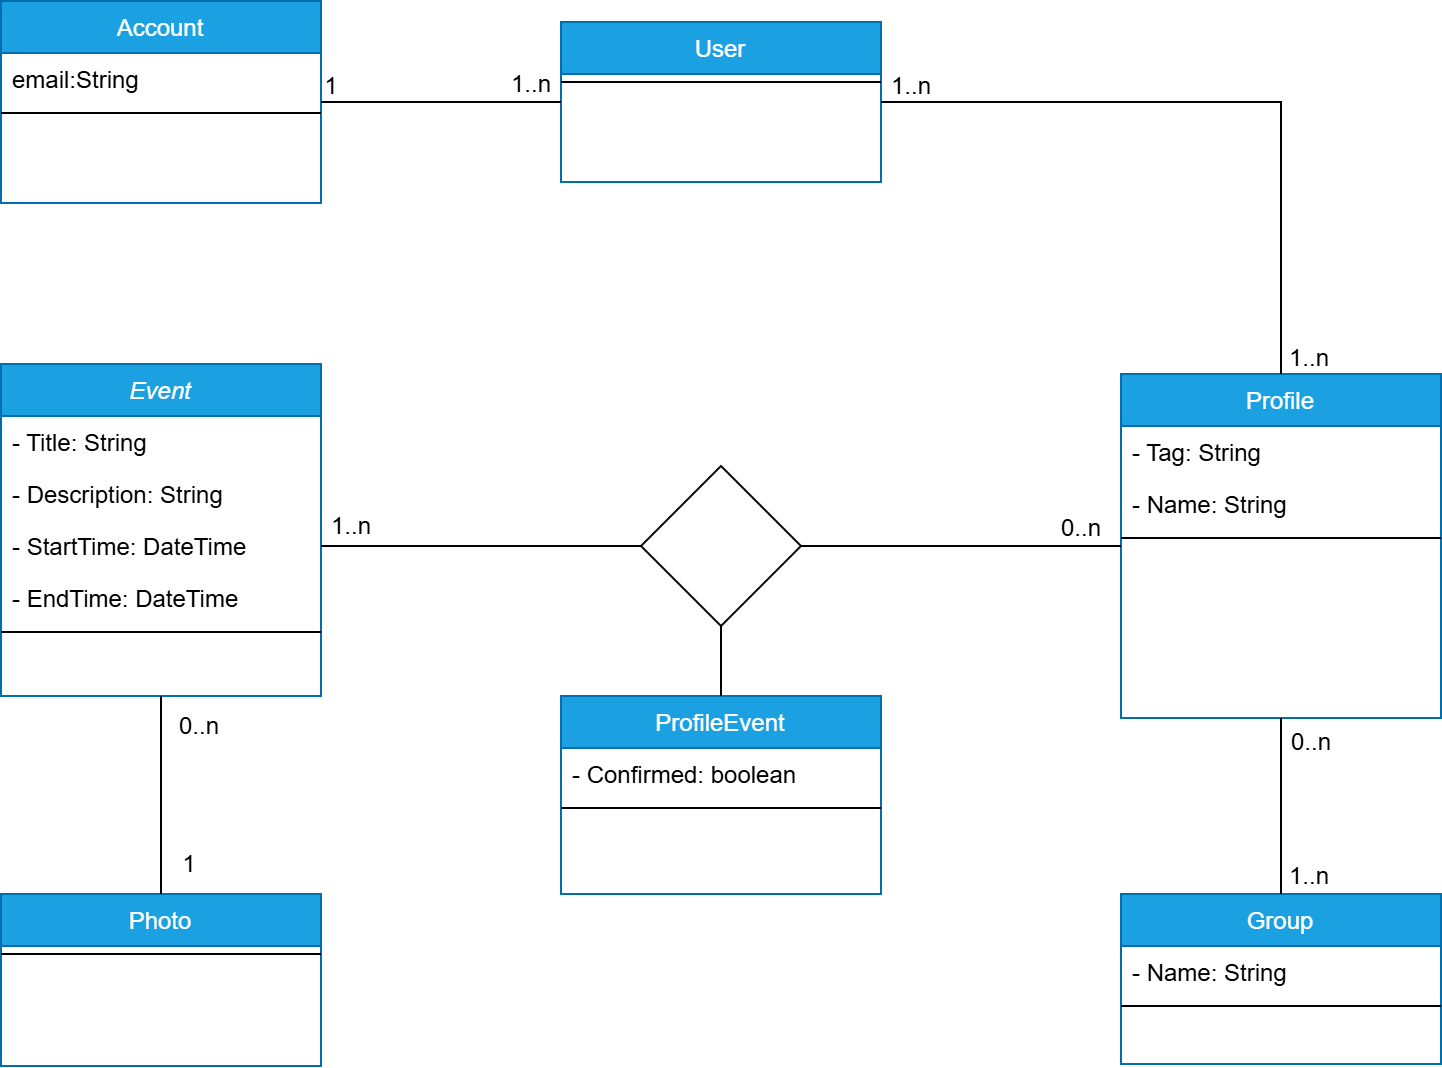
\includegraphics[width=\textwidth]{ModelloDominio.png}
        \caption{Modello del dominio}
    \end{center}
\end{figure}
\clearpage


Il diagramma dei package descrive la divisione delle responsabilità logiche.\\
Ogni package rappresenta una parte di prodotto che soddisfa una determinata responsabilità. 
La responsabilità viene individuata in base alla peculiarità ed alle dipendenze delle funzionalità che ricopre.
Si possono così distinguere, ad esempio, package relativi ad interfacce grafiche, logiche applicative o gestione della persistenza, 
in base alle caratteristiche specifiche del prodotto.
Il diagramma dei package offre una prima struttura delle parti del progetto e del loro rapporto.\\
\\

\begin{figure}[h!]
    \begin{center}
        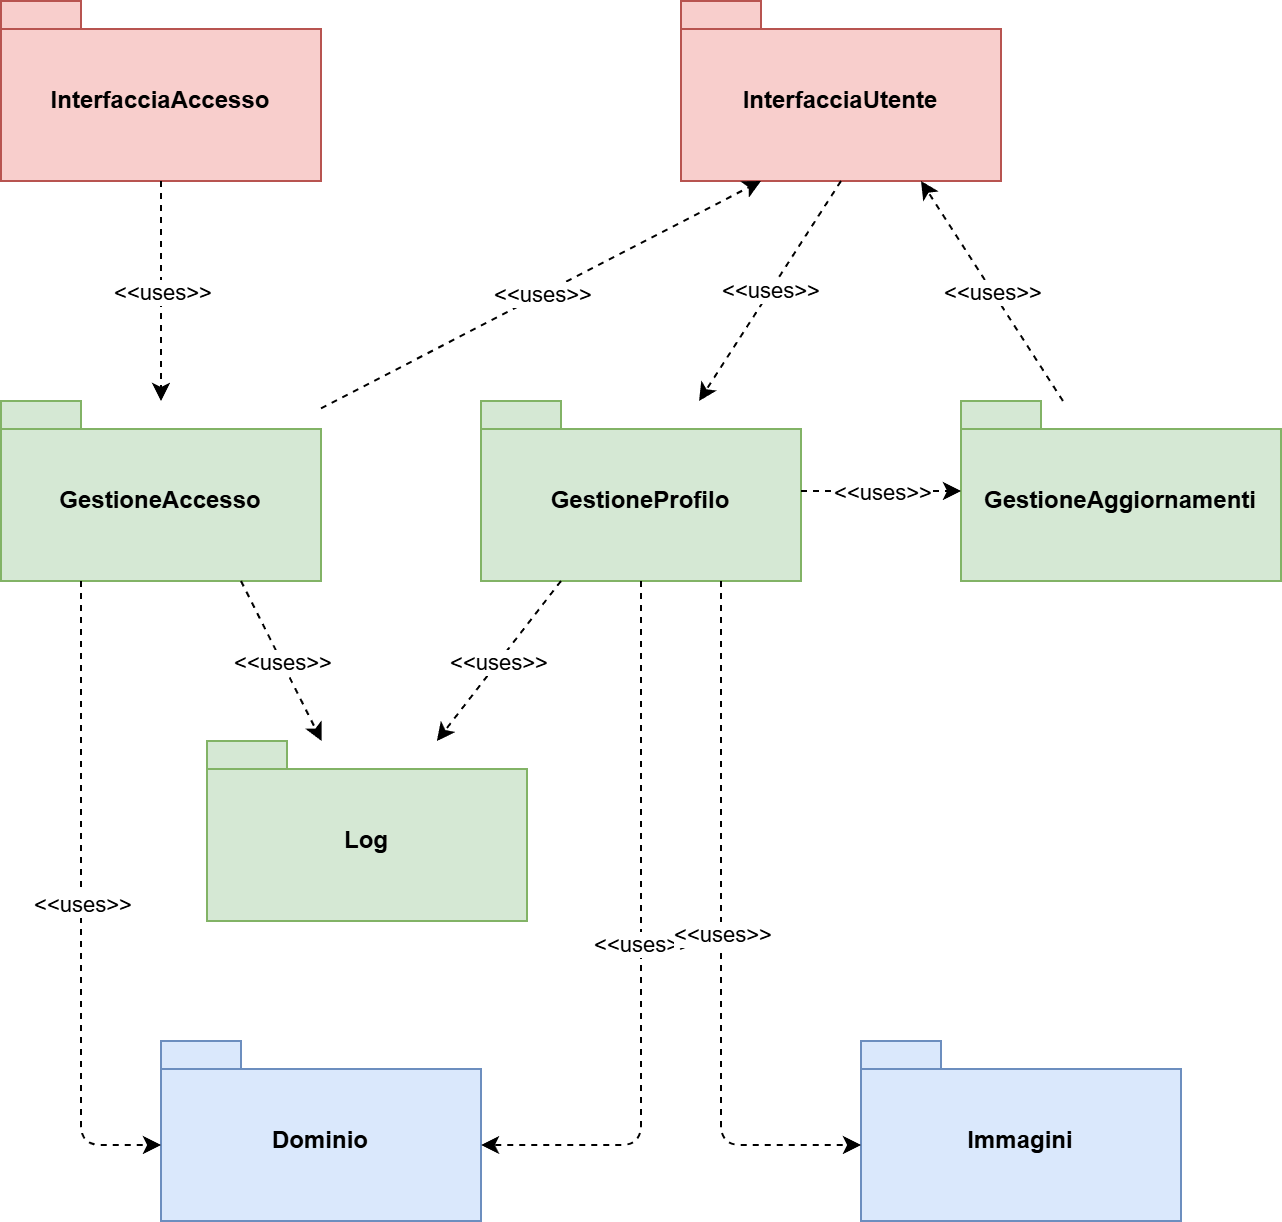
\includegraphics[width=\textwidth]{DiagrammaPackage.png}
        \caption{Diagramma dei Package}
    \end{center}
\end{figure}
\clearpage

Ogni package contiene una o più classi che lo implementano.
Ogni classe rappresenta un componente logico che assume uno specifico scopo.
Le classi possono presentare dei metodi, ovvero delle istanze che descrivono le funzionalità fornite,
alle quali altri componenti possono fare richiesta di esecuzione.
La definizione delle classi permette di creare una struttura iniziale presentando le funzionalità minime e 
le dipendenze tra le parti.\\

\begin{figure}[h!]
    \begin{center}
        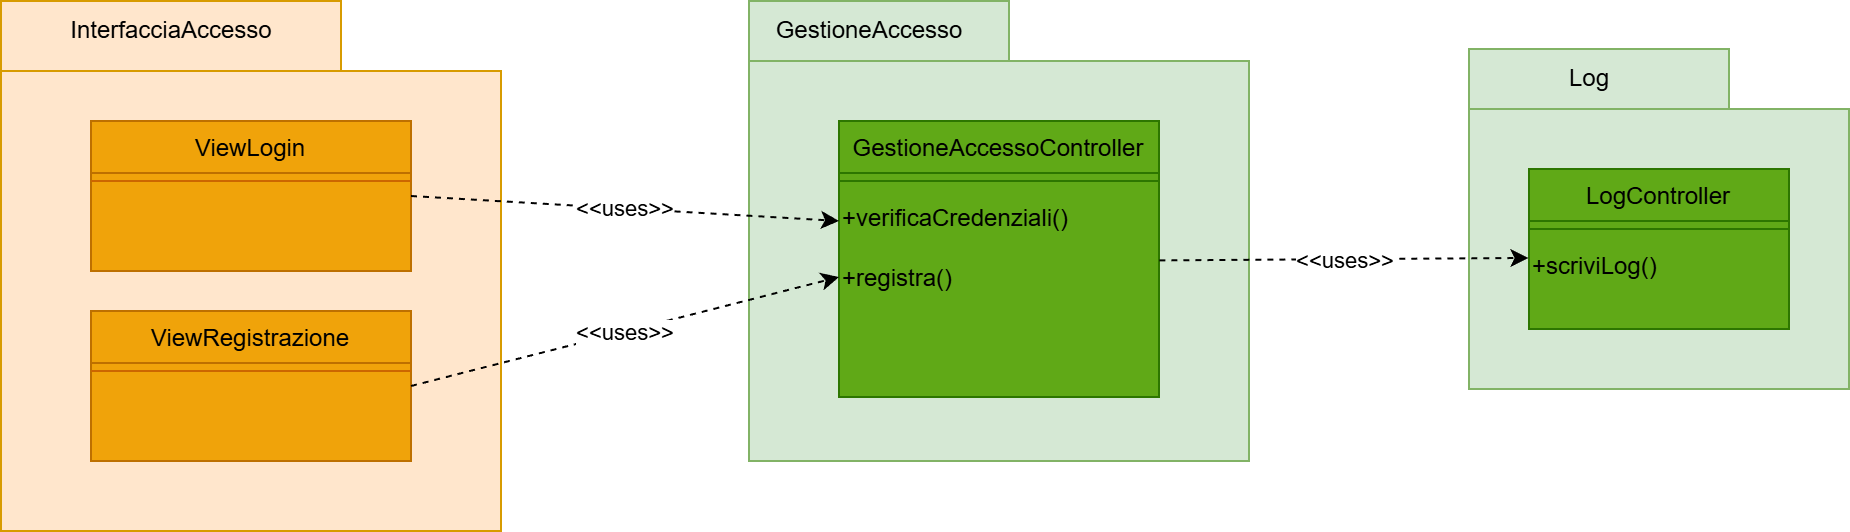
\includegraphics[height=0.18\textheight]{GestioneAccesso.png}
        \caption{Diagramma delle classi: interfacca e gestione accesso}
    \end{center}
\end{figure}


\begin{figure}[h!]
    \begin{center}
        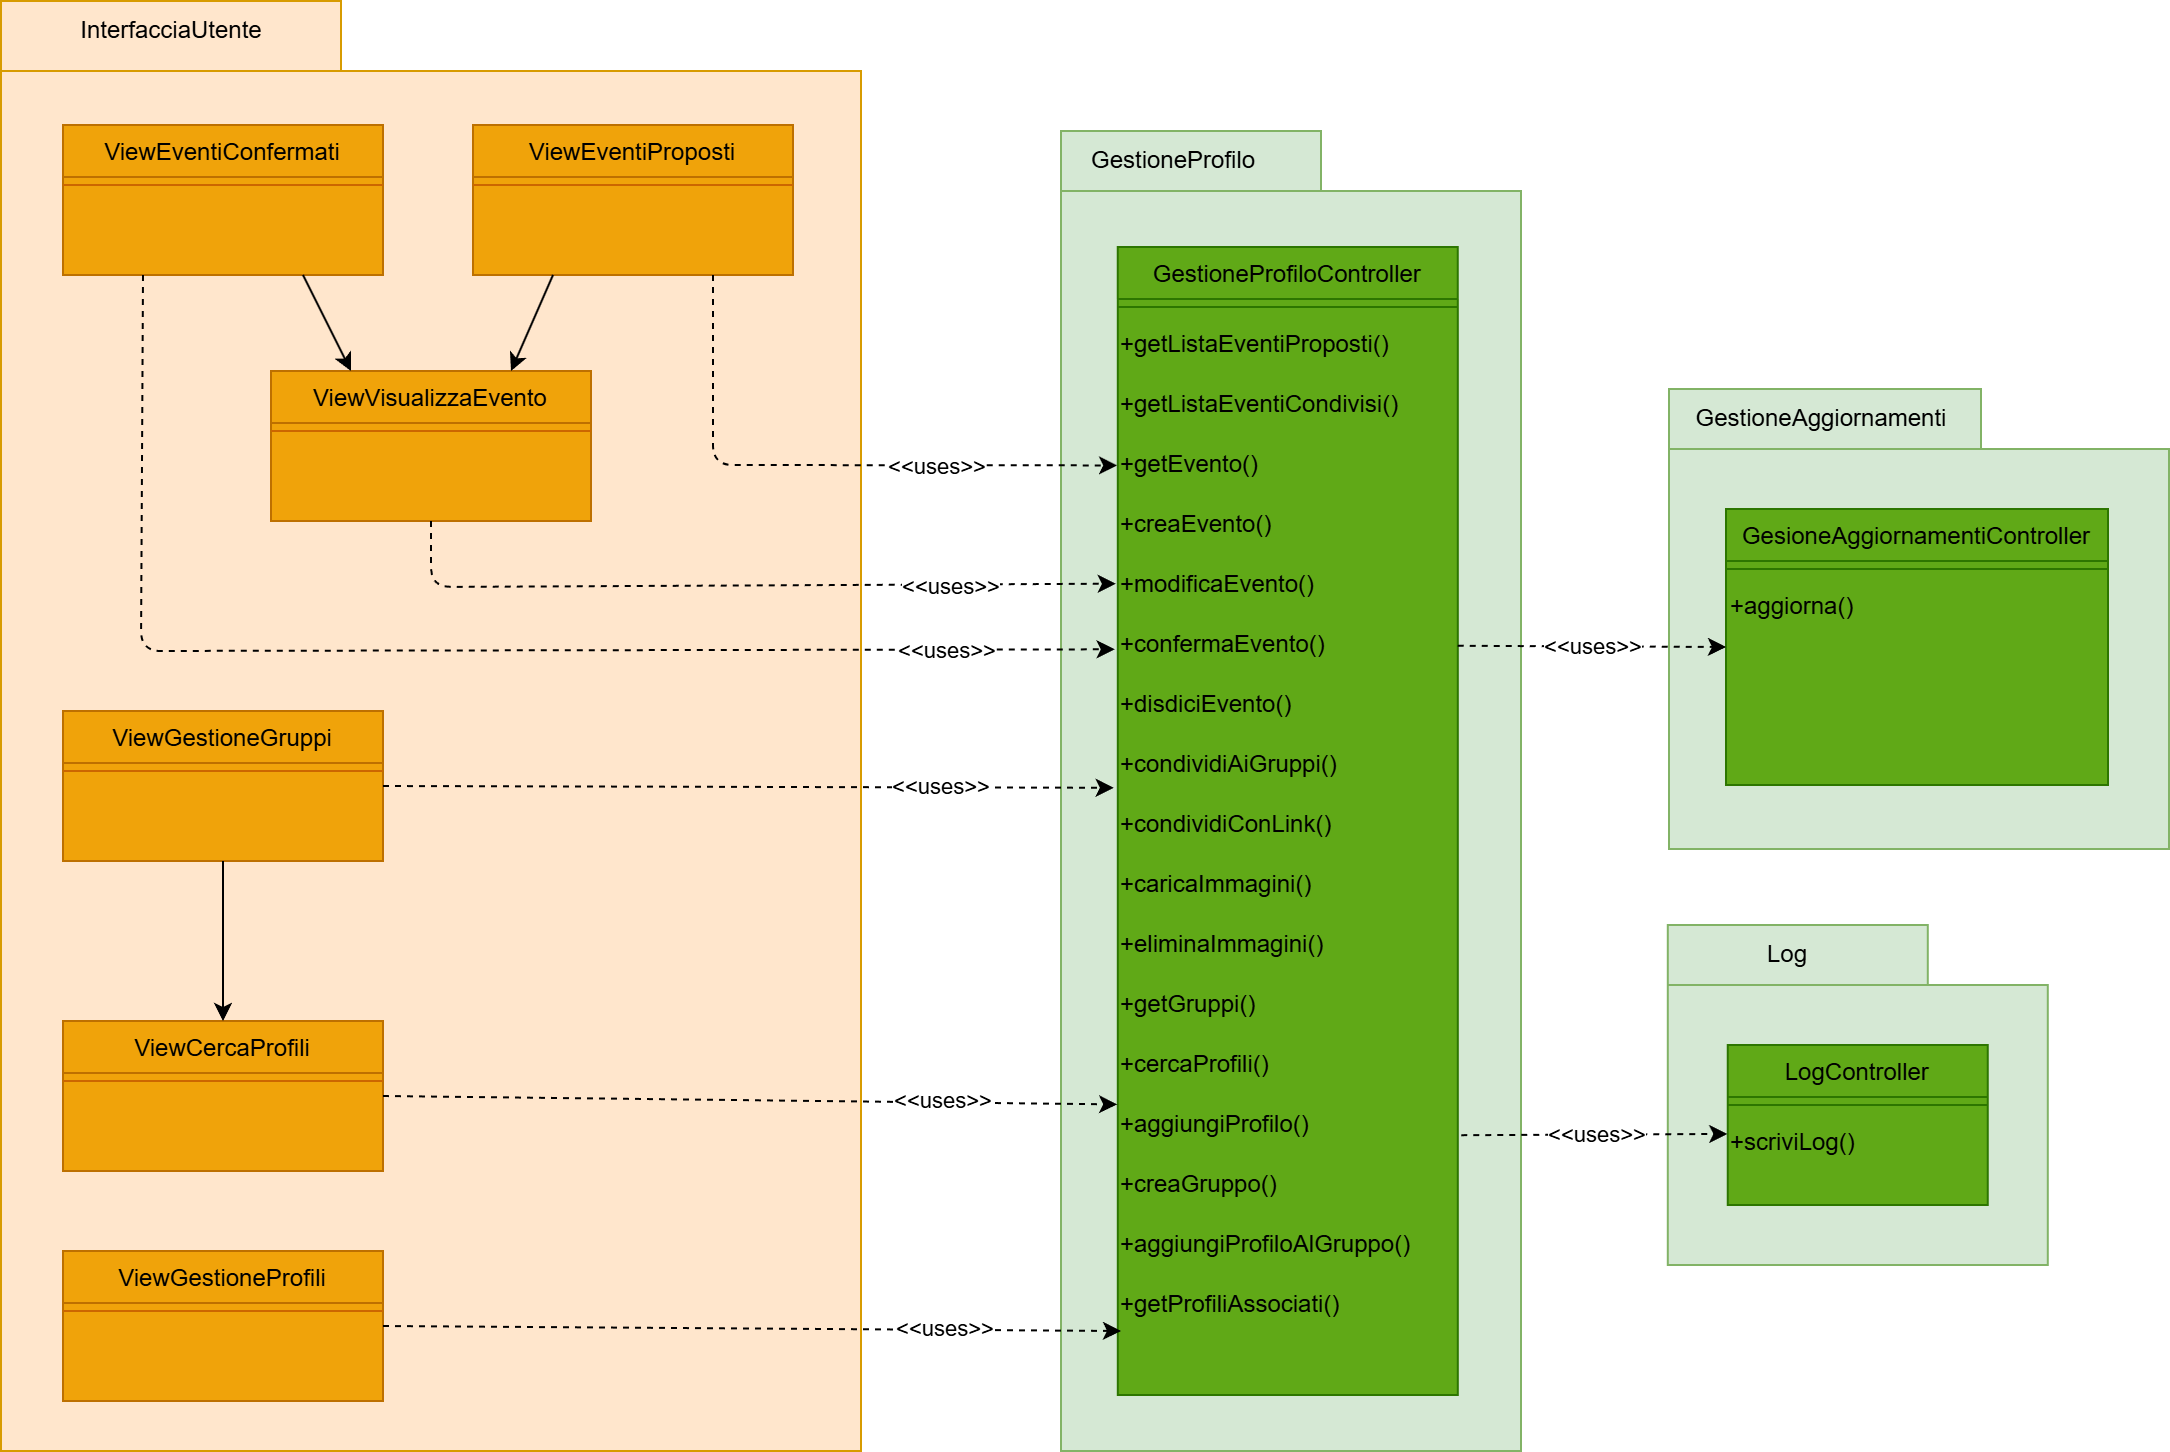
\includegraphics[height=0.425\textheight]{GestioneProfilo.png}
        \caption{Diagramma delle classi: interfacca utente, gestione profilo ed aggiornamenti}
    \end{center}
\end{figure}
\clearpage